\documentclass[fr]{../../../eplsummary}

\usepackage[SIunits]{../../../eplunits}

\usepackage{pgfplots}
\usepackage{xspace}

%\theoremstyle{definition}
%\newtheorem{mydef}{Définition}
%\newtheorem{mynota}[mydef]{Notation}
%\newtheorem{myprop}[mydef]{Propriétés}
%\newtheorem{myrem}[mydef]{Remarque}
%\newtheorem{myform}[mydef]{Formules}
%\newtheorem{mycorr}[mydef]{Corrolaire}
%\newtheorem{mytheo}[mydef]{Théorème}

\DeclareMathOperator{\res}{Res}
\DeclareMathOperator{\Arg}{Arg}
\DeclareMathOperator{\Log}{Log}
\DeclareMathOperator{\Atan}{atan2}

\hypertitle{Math\'ematique}{3}{FSAB}{1103}
{Gaetan Cassiers\and Beno\^it Legat\and Antoine Paris \and Louis Devillez}
{Jean-François Remacle, Grégoire Winckelmans et Roland Keunings}

\part{Equation aux dérivées partielles (EDP)}
\begin{myrem}
  \label{rem:inf}
  Ce cours traite des fonction qui ont un sens physique donc
  on a souvent besoin d'écrire que
  \[ \lim_{x\to\infty} u = \lim_{y\to\infty} u = 0. \]
  Ce n'est néanmoins pas tout le temps vrai.
  Par exemple, si $u$ est solution d'une équation de diffusion,
  vous ne pouvez pas dire que
  \[ \lim_{t\to\infty} u = 0 \]
  car l'intégrale de $u$ doit être conservée au cours du temps.

  Cependant, on peut tout le temps supposer que $u$ n'est jamais
  infini, même quand $t$ ou $x$ tendent vers l'infini.
  Sauf dans le cas d'un Dirac (voir annexe~\ref{app:dirac}), bien entendu.
\end{myrem}
\section{EDP du premier ordre}
Une EPD du premier ordre est une équation de la forme
\[ P(x, y)\fpart{u(x, y)}{x}
  + Q(x, y)\fpart{u(x, y)}{y}
  = R(x, y, u) \]
avec $P, Q, R$ des fonctions continues. % FIXME do I need it ?
$P$ et $Q$ peuvent aussi dépendre de $u$.
Dans ce cas,
on dit que l'EDP est \emph{quasi-linéaire} et
la méthode présentée ici ne marche pas toujours.
On va traiter un cas d'EDP \emph{quasi-linéaire}
dans la section~\ref{sec:burgers} où on s'en sort tout de même
car on a $R = 0$.

On remarque que l'équation se réécrit comme suit
\begin{equation}
  \label{eq:pqrn}
  \left(P, Q, R\right) \cdot \left(
  \fpart{u}{x}, \fpart{u}{y}, -1\right) = 0.
\end{equation}

Où $\left(\fpart{u}{x}, \fpart{u}{y}, -1\right)$ est connu pour être normal
à $u$ au point $\left(x, y, u(x, y)\right)$.
Par \eqref{eq:pqrn}, on a donc que $(P, Q, R)$ est perpendiculaire à la normale
c'est à dire qu'il est tangent au graphe de $u$.

$(P, Q, R)$ forme donc un champ de vecteur tangent au graphe de $u$.
Mais comment construire $u$ à partir de ce champ ?

On remarque que comme $P$, $Q$ et $R$ sont continues, deux vecteurs proches
seront presque parallèles. Le champ est donc composé de courbes l'une à côté
de l'autre.

Pour déterminer $u$, la technique est de commencer par trouver ces courbes
dans le plan $xy$ puis de leur ajouter leur hauteur $u$.
On appelle ces courbes les \emph{courbes caractéristiques}.

\subsection{Nécessité de conditions initiales}
On connait les tangentes à $u$, on sait donc construire une
sorte de coque mais à quelle hauteur mettre cette coque ?
Aussi, comment agencer ces courbes caractéristiques l'une à côté de l'autre.
En effet, le champ de vecteurs formé par $(P, Q, R)$ est formé de vecteurs
qui sont parallèles lorsqu'ils sont très proches.
Si on a nos courbes caractéristiques, notre coque est encore malléable,
on peut déplacer ces courbes de haut en bas par rapport à une autre.

En donnant une condition initiale qui coupe une et une seule fois chaque
courbe caractéristique, on détermine tout cela.
Notons $\Gamma$, cette courbe paramétrée en fonction de $s$
\[ \Gamma \equiv (x(s), y(s)). \]
On connait le long de cette courbe $u(x(s), y(s)) = f(s)$.

\subsection{Détermination des courbes caractéristiques}
\label{sec:detcara}
On cherche une courbe dont $(P, Q)$ est tangent c'est à dire que
\[ \fdif{y}{x} = \frac{Q}{P} \]
Le long de ces courbes, on a donc
\[ P(x, y)\dif y = Q(x, y) \dif x. \]
Il peut être judicieux ici de se retrouver avec que du $y$ à gauche
et que du $x$ à droite
\begin{align*}
  P'(y) \dif y & = Q'(x) \dif x & \frac{P'(y)}{Q'(x)} = \frac{P(x,y)}{Q(x,y)}.
\end{align*}
Pour déterminer ces courbes, il nous faut utiliser la condition initiale, donc
\[ \int_{y' = y(s)}^{y' = y} P'(y') \dif y'
= \int_{x' = x(s)}^{x' = x} Q'(x') \dif x' \]
où $x'$ et $y'$ sont des variables introduites juste pour l'intégration
car on a déjà $x$ et $y$ aux bornes donc on ne peut pas les utiliser pour
intégrer.

On arrive donc à une équation $g_s(x, y) = 0$ que $x$ et $y$ doivent
respecter pour être sur la courbe caractéristique passant par $(x(s), y(s))$.

\subsection{Détermination de $u$ le long des courbes caractéristiques}
On doit maintenant déterminer $u$ le long de ces courbes.
Pour ce faire, on va réutiliser le champ de vecteur $(P, Q, R)$ et sa
tangence au graphe de $u$.
On va intégrer \emph{le long d'une caractéristique} où on a
une équation $g_s(x, y) = 0$ qu'on a trouvé au point précédent
qui est respectée
\begin{align*}
  P \dif u & = R \dif x\\
  Q \dif u & = R \dif y.
\end{align*}
Ces deux équations sont équivalentes car, comme on est le long des
caractéristiques où $P \dif y = Q \dif x$.

On peut maintenant choisir la plus simple.
Sans perte de généralité, disons que c'est la première et
on va faire la même manipulation qu'au point précédent
\[ P'(u) \dif u = R'(x, y) \dif x. \]
On peut maintenant utiliser la condition initiale $u(s)$ pour
déterminer la hauteur des courbes caractéristiques
\[ \int_{u' = f(s)}^{u' = u(x,y)} P'(u') \dif u'
= \int_{x' = x(s)}^{x' = x} R'(x', y_s(x')) \dif x'. \]
où $y_s(x')$ est la valeur de $y$ lorsque $x = x'$
sur la courbe caractéristique respectant $g_s(x, y) = 0$.

\begin{myrem}[$s$ est constant]
  Il est important de bien réaliser que, lors de l'intégration,
  $s$ est bien constant et ne dépend pas de $x'$.
  On intègre sur \emph{une} caractéristique
  (celle qui passe par $(x(s), y(s))$ et qui respectent donc
  $g_s(x', y') = 0$), c'est d'ailleurs pour insister sur cela que je mets
  $s$ en indice de $g$ et pas en argument.
  Il est d'ailleurs inutile de développer $f(s)$ ici si on nous donne
  son équation.
\end{myrem}

On arrive à une équation de $u(x, y)$ dépendant de $x$ et $s$.
Il faut maintenant isoler $s$ dans la condition $g_s(x, y) = 0$ et trouver
$s(x, y)$.
On remplace alors, dans l'expression de $u(x, y)$, $s$ par $s(x, y)$.

\subsection{Equation de transport (ou de convection)}
On peut écrire de manière générale l'équation de transport de la façon
suivante

$$c\fpart{u}{x} + \fpart{u}{t} = 0$$

Où $c$, dans le cas d'un problème physique, est une vitesse. $c$ peut être
une constante, une fonction de $x$ (cas du transport dans un milieu non-homogène),
ou une fonction de $t$. $c$ peut même être une fonction de $u$, dans ce cas
l'EDP n'est plus linéaire, nous traiterons un exemple d'équation de transport
non-linéaire dans la section \ref{sec:burgers}. Comme l'équation est homogène,
$u$ est conservée le long des caractéristiques et ce genre d'équation est assez
simple à résoudre.

\subsubsection{Equation de transport sous-forme conservative}
Une autre forme de l'équation de transport est la forme conservative :

$$\fpart{}{x}(cu) + \fpart{u}{t} = 0$$

où $c = c(x,t,u)$ (on remarque que dans le cas $c$ constant ou $c = c(t)$,
on revient au cas précédent). L'équation sous forme conservative est telle
que l'intégrale de $u$ est conservée au cours du temps. C'est donc souvent
ce type d'équation qu'on rencontre en physique. Pour résoudre cette équation
par la méthode des caractéristiques, il faut d'abord la développer

$$c\fpart{u}{x} + \fpart{u}{t} = -\fpart{c}{x}u.$$

\subsubsection{Equation de transport non-linéaire}
\label{sec:burgers}
\begin{myrem}
	L'équation de densité de transport non-linéaire n'a pas été vue lors de
	l'année 2016-2017.
\end{myrem}
La forme générale de l'équation de transport non-linéaire est

$$c(u)\fpart{u}{x} + \fpart{u}{t} = 0.$$

avec comme condition initiale, par exemple, $u(s, 0) = f(s)$.
Cependant, nous considérons dans ce cours un cas particulier, appelé
équation de \textit{Burgers}, dans lequel $c(u) = u$.
Les caractéristiques sont obtenues par intégration de

$$\dif x = u\dif t.$$

Comme l'équation de Burgers est homogène, $u$ est conservée
le long des caractéristiques et on a des caractéristiques de la forme
$x = s + f(s)t$. On constate assez facilement que les pentes des
caractéristiques dépendent de $s$, elles sont donc variables. Cela
peut poser problème car des caractéristiques peuvent se croiser, la
solution deviendra alors discontinue. On peut démontrer assez facilement
que le temps critique pour l'apparition de la discontinuité correspond
au minimum de $\frac{-1}{\fdif{f}{s}}$. Cette fonction est minimum
lorsque $\ffdif{f}{s}$ s'annule.

\subsection{Équation de densité de traffic}
\begin{myrem}
	L'équation de densité de traffic n'a pas été vue lors des
	années 2014-2017. Cependant elle est assez intéressante et permet
	d'avoir un exemple concret d'utilisation d'une EDP (et plus précisément
	d'une équation de transport sous forme conservative).
\end{myrem}

\label{sec:traffic}
Soit
\begin{itemize}
  \item $\rho(x, t)$, le nombre de véhicules par mètre
    en $x$ au temps $t$;
  \item $u(x, t)$, la vitesse des véhicules en $x$ au temps $t$;
  \item $N(x_0, x_1, t)$, le nombre de véhicules entre $x_0$ et $x_1$
    au temps $t$.
\end{itemize}
On peut écrire
\begin{align}
  \label{eq:Nrho}
  N(x_0, x_1, t) & = \int_{x_0}^{x_1} \rho(x, t) \dif x\\
  \nonumber
  \fpart{N}{t} & \stackrel{\eqref{eq:Nrho}}{=}
  \int_{x_0}^{x_1} \fpart{\rho(x, t)}{t} \dif x\\
  \nonumber
  \fpart{N}{t} & = u(x_0, t) \rho(x_0, t) - u(x_1, t) \rho(x_1, t)\\
  \nonumber
  & = - \int_{x_0}^{x_1} \fpart{(u\rho)}{x} \dif x.
\end{align}
D'où
\[ \int_{x_0}^{x_1} \fpart{\rho}{t} + \fpart{(u\rho)}{x} \dif x = 0. \]
Comme c'est vrai pour tout intervalle $[x_0, x_1]$, on a
\begin{equation}
  \label{eq:traffic}
  \fpart{\rho}{t} + \fpart{(u\rho)}{x} = 0.
\end{equation}

\subsubsection{Le modèle de Lighthill-Whitham-Richards}
En utilisant le modèle de Lighthill-Whitham-Richards qui
se résume à dire qu'il y a une vitesse et une densité maximale
et que la vitesse diminue linéairement avec la densité du trafic,
autrement dit
\[ u(\rho) =
u_\mathrm{max} \left(1 - \frac{\rho}{\rho_\mathrm{max}}\right) \]
on peut réécrire l'équation~\eqref{eq:traffic} en fonction de $\rho$
en observant que
$\fpart{(u(\rho)\rho)}{x} = \fpart{(u(\rho)\rho)}{\rho}\fpart{\rho}{x}$.

On obtient
\[ \fpart{\rho}{t} + u_\mathrm{max}
\left(1 - \frac{2\rho}{\rho_\mathrm{max}}\right)\fpart{\rho}{x} = 0 \]
où le facteur devant $\fpart{\rho}{x}$ peut être interprété comme la vitesse
de l'\emph{information} car on sait par la méthode des caractéristiques
qu'il vaut la pente des caractéristiques $\fdif{x}{t}$.

La technique vue à la section~\ref{sec:detcara} en marche
pas car $Q$ est en fonction de $\rho$ et pas que de $x$ et $t$.
Seulement, les caractéristiques sont tout de même des droites
car, comme l'équation est homogène,
$\rho$ ne varie pas le long des caractéristiques et cette
pente est donc constante et vaut
\[ \fdif{x}{t} =
u_\mathrm{max} \left(1-\frac{2\rho(s)}{\rho_\mathrm{max}}\right). \]
On remarque que cette vitesse est \emph{négative} si
$\rho > \frac{\rho_\mathrm{max}}{2}$,
en effet, c'est la vitesse de l'\emph{information} et non
des voitures.

\paragraph{Intersection des caractéristiques}
Le problème c'est que si, dans la conditions initiale,
il y a un traffic dégagé suivit d'un traffic dense,
il y aura un choc des caractéristiques.
Cette endroit de choc sera une discontinuité dans la densité du traffic,
on passera de caractéristiques voulant que le traffic soit dégagé à des
caractéristiques voulant un traffic dense.
Ça peut s'apparenter à des voitures rencontrant un bouchon.

Si il y a une discontinuité dans le traffic en $x_0$ au départ,
comme dans le cas d'un feu rouge,
\[ \rho_-(x_0) > \rho_+(x_0) \]
on a une zone où aucune caractéristique ne vient donner d'information
car la vitesse de l'information en $x_0$ à gauche est plus petite
que celle à droite.
Il faut alors considérer que toutes les densités de l'intervalles
$[\rho_-(x_0); \rho_+(x_0)]$ se trouvent au point $x_0$.
Ainsi, on peut faire partir toutes les caractéristiques correspondantes
du point $x_0$ et on peut recouvrir cet intervalle.

\section{EDP du second ordre}
Une EPD du deuxième ordre est une équation de la forme
\[ A \ffpart{\phi}{x} + B\fdpart{\phi}{x}{y} + C\ffpart{\phi}{y} = R \]
où $A$, $B$, $C$ et $R$ sont des fonction régulière qui peuvent
dépendre de $x$, $y$, $\phi$ ou même de $\fpart{\phi}{x}$ ou de
$\fpart{\phi}{y}$. On suppose que l'on dispose de $\phi(\Gamma(s))$ et
$\fpart{\phi}{n}(\Gamma(s))$ le long de la courbe paramétrée $\Gamma
\equiv (x(s), y(s))$, avec $n(s)$ la direction normale à $\Gamma$.

Le problème est bien posé si et seulement si
\[
  \begin{vmatrix}
    A & B & C\\
    \fdif{x}{s} & \fdif{y}{s} & 0\\
    0 & \fdif{x}{s} & \fdif{y}{s}
  \end{vmatrix}
  \neq 0.
\]

On distingue les EDP de second ordre en 3 cas
\begin{center}
  \begin{tabular}{|l|l|}
    \hline
    $B^2 - 4AC > 0$ & EDP hyperbolique\\
    $B^2 - 4AC = 0$ & EDP parabolique\\
    $B^2 - 4AC < 0$ & EDP elliptique\\
    \hline
  \end{tabular}
\end{center}

\subsection{Équation d'onde}
Une équation d'onde est une EDP hyperbolique dont l'équation est
\[ c^2 \lap \phi = \ffpart{\phi}{t}. \]
Avec deux conditions initiales : $\phi(x, y, t=0) = \phi_0(x, y)$ et
$\fpart{\phi}{t}(x, y, t=0) = \phi'(x, y)$.

En 1D, ça devient
\[ c^2\ffpart{\phi}{x} - \ffpart{\phi}{t} = 0. \]
avec les conditions initiales $\phi(x, t=0) = f(x)$ et $\fpart{\phi}{t}(x, t=0) = g(x)$.

La formule d'\textit{Alembert} nous permet alors d'arriver à
\[ \phi(x, t) = \frac{1}{2}(f(x - ct) + f(x + ct)) + \frac{1}{2c}\int_{x-ct}^{x+ct}
g(x')\dif x'\]

Dans le cas $g=0$, cette formule nous permet de trouver graphiquement $\phi$ à un temps
$t$ à partir du réseau des caractéristiques et de $f(s)$.

% TO DO : zone de dépendance et zone d'influence (voir figure dans le correctif
% de l'APE3), ajouter la démonstration de la formule d'Alembert
% en annexes?

\subsection{Équation de diffusion}
Une équation de diffusion est une EDP parabolique dont l'équation est
\[ \alpha \lap \phi = \fpart{\phi}{t} \]
où $\alpha$ est le coefficient de \emph{diffusivité}.

En 1D, ça devient
\[ \alpha \ffpart{\phi}{x} = \fpart{\phi}{t}. \]

On remarque qu'on a ici besoin d'une seule condition initiale $\phi_0(x, y)$
puisque $\fpart{\phi}{t}(x, y, 0) = \lap \phi(x, y, 0) = \lap \phi_0(x, y)$.
La deuxième condition est donc donnée par l'EDP elle même.

\begin{myrem}[unités de $\alpha$]
  On remarque que comme $\lap \phi$ a des unités de $[\phi]\per\meter\squared$
  et que $\fpart{\phi}{t}$ a des unités de $[\phi]\per\second$,
  $\alpha$ doit avoir des unités de $\meter\squared\per\second$.
\end{myrem}

L'équation de diffusion étale une fonction de départ en gardant
l'intégrale constante.
Elle perd tous les détails de la fonction de départ et n'est donc
pas réversible, c'est à dire que lorsqu'on connait $\phi(t)$, on
peut connaitre $\phi(t + \Delta t)$ uniquement si $\Delta t \geq 0$.

Si la fonction de départ est un Dirac (voir annexe~\ref{app:dirac})
\[ \phi(x, 0) = Q \delta(x). \]
La solution est une gaussienne
\[ \phi(x, t) = \frac{Q}{\sqrt{\pi4\alpha t}}
\exp\left(-\frac{x^2}{4\alpha t}\right). \]
Si la fonction de départ est une gaussienne
\[ \phi(x, 0) = \phi_0 \exp\left(-\frac{s^2}{b^2}\right), \]
on peut imaginer qu'elle vienne d'un Dirac
\footnote{On n'est pas sûr que ça soit vrai,
comme dit précédemment, une diffusion n'est pas réversible.
Il pourrait y avoir plus de détails qui
ont été effacés mais considérer l'un ou l'autre ne change rien
si on s'intéresse au futur.}.
On a alors nécessairement
\begin{align*}
  b^2 & = 4\alpha t\\
  \phi_0 & = \frac{Q}{\sqrt{\pi4\alpha t}}
\end{align*}
d'où
\[ \phi(x, t) = \frac{\phi_0b}{\sqrt{b^2 + 4\alpha t}}
\exp\left(-\frac{x^2}{b^2 + 4\alpha t}\right). \]

Cela permet de trouver la solution pour n'importe quelle condition initiale,
que l'on considère comme une somme de Dirac :
$\phi_0(x) = \int_{-\infty}^\infty \phi_0(x')\delta(x-x') \dif x'$.
La solution est alors la somme des solutions pour tous les Dirac considérés :
\[\phi(x, t) =
    \int_{-\infty}^{\infty} \frac{\phi_0(x')}{\sqrt{\pi 4\alpha t}}
    \exp\left(-\frac{(x-x')^2}{4\alpha t}\right) \dif x'
\]

\begin{myrem}
L'équation d'onde et l'équation de diffusion sont résolues ici dans
le cas d'un domaine infini, ils sont alors donnés en condition initiale :
$\phi(x, y, t=0)$ est donné sur tout le domaine (et aussi
$\fpart{\phi}{t}(x, y, t=0)$ pour l'équation d'onde). Si le domaine
est borné, il faut imposer en plus une condition limite sur la frontière
du domaine, l'équation se résout alors par séparation des variables
(sous certaines conditions).
\end{myrem}

\subsection{Équation de Laplace}
Une équation de Laplace est une EDP elliptique dont l'équation est
\[ \lap \phi = 0. \]
En 2D, ça devient
\[ \ffpart{\phi}{x} + \ffpart{\phi}{y} = 0. \]
Elle se résout à l'aide d'une séparation des variables
(voir section~\ref{sec:sepvar}).

% TODO : lien entre équation de diffusion et équation de Laplace
% Voir exemple de diffusion thermique donné en cours.
% Propriétés fondamentales de l'éq. de Laplace : théorème
% de la moyenne

\subsection{Équation de Poisson}
Une équation de Poisson est une EDP elliptique dont l'équation est
\[ \lap \phi = R. \]
En 2D, ça devient
\[ \ffpart{\phi}{x} + \ffpart{\phi}{y} = R. \]
On remarque que l'équation de Laplace est le cas particulier de
l'équation de Poisson où $R = 0$.

\section{Méthode de séparation de variables}
\label{sec:sepvar}
Nous nous intéressons ici à la méthode de séparation des variables pour les EDP
qui n'est pas la même que celle pour les EDO.

On va supposer qu'il existe deux fonctions $X$ et $Y$ telles que
\[ \phi(x, y) = X(x) \cdot Y(y). \]
À partir de cette supposition, il est maintenant possible de résoudre
les EDP plus facilement.

Pour que cette méthode marche, il faut deux choses
\begin{itemize}
  \item L'équation doit être homogène et linéaire;
  \item Le domaine doit se ramener à un domaine rectangulaire
    (ou cubique si on est en 3D)
    avec, si nécessaire, un changement de variable.
\end{itemize}
Pour la 2\ieme{} condition, un changement de variable classique est
celui pour passer d'un cercle à un carré
\[ (x, y) = (r\cos\theta, r\sin\theta). \]
Dans ce cas,
\begin{align*}
  \lap \phi & = \ffpart{\phi}{x} + \ffpart{\phi}{y}\\
  & = \ffpart{\phi}{r} + \frac{1}{r}\fpart{\phi}{r}
  + \frac{1}{r^2}\ffpart{\phi}{\theta}
\end{align*}

Sur les côtés, on pose des conditions limite.
Ces conditions sont soit homogènes, soit non-homogènes.
Elles sont de 3 types:
\begin{itemize}
  \item Conditions de Dirichlet,
    on impose une condition sur $\phi$;
  \item Condition de Neumann,
    on impose un condition sur $\fpart{\phi}{v}$ pour
    une certaine variable $v$;
  \item Condition de Robin,
    on impose une condition sur une combinaison linéaire de
    $\phi$ et $\fpart{\phi}{v}$ pour une certaine variable $v$.
\end{itemize}

On peut aussi appliquer la méthode de séparation des variables
avec un domaine infini, dans ce cas il peut être utile
de se souvenir de la remarque~\ref{rem:inf}, c'est à dire
que que $u$ ne peut pas tendre vers l'infini,
pour éliminer une des exponentielles qu'on obtient.

\subsection{L'équation de Laplace par séparation de variables}
Supposons qu'on soit dans un rectangle.
Il nous faut 4 conditions limites, une sur chaque côté.
Si toutes les conditions limites sont homogènes, la solution est la solution
triviale $\phi = 0$.

On ne sait gérer qu'une seule condition limite non-homogène à la fois.
S'il y en a plusieurs, on les traite séparément en prenant les autres
égales à 0 puis on somme les solutions.
En effet, comme l'équation de Laplace est linéaire, le principe
de superposition s'applique.
Supposons donc par la suite qu'on ait une seule condition limite non-homogène.

\subsubsection{Recherche des solutions}
On peut calculer
\[ \lap \phi = X'' Y + X Y''. \]
On a donc, dans le cas de l'équation de Laplace,
\[ \frac{X''}{X} + \frac{Y''}{Y} = 0 \]
où on a divisé par $XY$ car on les suppose non-nuls comme on
écarte la solution triviale.

En dérivant l'équation par $x$, on a
\[ \fdif{\left(\frac{X''}{X}\right)}{x} + 0 = 0 \]
d'où on tire que $\frac{X''}{X}$ est égal à une constante $\pm k^2$
et donc $\frac{Y''}{Y} = \mp k^2$.
On a ici 3 cas à traiter où on pose $k > 0$
\begin{itemize}
  \item $X'' = k^2X$ qui donne une solution $\phi_1 = X_1Y_1$
    avec $X_1 = Ae^{kx} + Be^{-kx}$ et $Y_1 = C\cos(ky) + D\sin(ky)$;
  \item $X'' = -k^2X$ qui donne une solution $\phi_2 = X_2Y_2$
    avec $X_2 = E\cos(kx) + F\sin(kx)$ et $Y_2 = Ge^{ky} + He^{-ky}$;
  \item $X'' = 0$ qui donne une solution $\phi_3 = X_3Y_3$
    avec $X_3 = Ix + J$ et $Y_3 = Ky + L$.
\end{itemize}

\subsubsection{Application des conditions limites homogènes}
Posons $\phi_\Sigma = \phi_1 + \phi_2 + \phi_3$.
Que doit-on faire maintenant ?
Appliquer les conditions sur $\phi_1$, $\phi_2$ et $\phi_3$ séparément ou
sur $\phi_\Sigma$ ?
Rappelons nous que rien ne nous indiquait que $\phi$ était effectivement
à variable séparable.
Ici, on a trouvé $\phi_1$, $\phi_2$ et $\phi_3$ qui respectent
l'équation de Laplace, $\phi_\Sigma$ la respecte aussi mais n'est plus
à variable séparable.

Comme rien ne nous impose que $\phi$ soit à variable séparable,
dans le cas général, il faut appliquer les conditions limites sur
$\phi_\Sigma$ et non sur $\phi_1$, $\phi_2$ et $\phi_3$ séparément sinon
on se rajoute une contrainte qui n'existe pas et on perd potentiellement
des solutions.
Seulement, dans la plupart des cas, ça ne change rien
de le faire séparément ou non et ça complique énormément les calculs.
En pratique, une bonne manière de faire est donc d'appliquer
les conditions limites séparément et si plus aucune solution
ne subsiste, appliquer les conditions limites sur $\phi_\Sigma$.
En effet, on a déjà potentiellement perdu des solution avec la supposition
que $\phi$ était à variable séparable, pourquoi ne pas continuer
sur notre lancée ?

En appliquant les conditions limites séparément,
pour les conditions limites homogènes,
on arrive à des équations du style
\[ u(x, 0) = 0 = X(x)Y(0). \]
Si $X(x) = 0$ pour tout $x$, on a la solution triviale, comme elle
est inintéressante, supposons que $\exists x$ tel que $X(x) \neq 0$ et donc
on a $Y(0) = 0$.
Une des deux variables a deux conditions homogènes,
ça permet d'éliminer deux solutions.
Par exemple, si c'est $X$ qui a deux conditions homogènes,
on arrive nécessairement à $X_1 = X_3 = 0$
donc $\phi_1$ et $\phi_3$ sont triviaux.

On remarque ici que $\phi_3$ est éliminé dans les deux cas.
En effet, il n'est que utile dans le cas où on applique
les conditions limites sur $\phi_\Sigma$.
Il peut être utile par exemple dans un cas de domaine semi infini où
on veut que $\phi$ ne tende pas vers 0.
Les exponentielles sont alors inutiles car elle tendent
soit vers l'infini, soit vers 0
et les cosinus et les sinus ne convergent pas.
Dans ce cas, si on applique les conditions limite séparément,
on ne trouvera pas de solution, il faudra
l'appliquer sur $\phi_\Sigma$ et on ne trouvera pas un $\phi_3$ nul.
On dira alors que $\phi_3$ est la solution en régime.
$\phi_1 + \phi_2$ est alors la solution transitoire.

En continuant dans notre exemple avec les deux
conditions homogènes en $x$, supposons que les deux
conditions soient $u(0, y) = 0$ et $u(L, y) = 0$.
On a alors
\begin{align*}
  E & = 0\\
  E\cos(kL) + F\sin(kL) & = 0
\end{align*}
D'où, soit $F = 0$, soit $\sin(kL) = 0$, le premier cas nous
donne la solution triviale, ce qui ne nous intéresse pas.
Le deuxième cas nous restreint les possibilités de $k$,
en se souvenant qu'on a posé que $k > 0$, à
\begin{align*}
  k_n & = \frac{n\pi}{L} & n = 1, 2, \ldots
\end{align*}

Complétons maintenant chacune de ces solution avec la solution
associée pour $Y$.
On a à résoudre
\[ Y_n'' = k_n^2Y_n \]
il est important d'utiliser $k_n$ ici et non $k$
car $X''/X$ et $-Y''/Y$ valent la même constante.

À nouveau, rien ne nous oblige que $\phi$ soit à variable
séparable et en l'imposant on risque de perdre des solutions.
Par le principe de superposition,
la solution générale s'écrit donc maintenant,
\[ \phi(x,y) = \sum_{n=0}^{n=\infty} F_n \sin(k_nx)Y_n(y). \]

\subsubsection{Application de la condition limite non-homogène}
L'astuce, ici, c'est de remarquer que les sinus
forment une base orthogonale avec le produit vectoriel
\[ \int_{x = 0}^{x = L} \sin\left(\frac{n\pi}{L} x\right)
\sin\left(\frac{m\pi}{L} x\right) \dif x. \]
En effet, si $n \neq m$, ce produit vectoriel est nul et
si $n = m$, il vaut $\frac{L}{2}$.

Utilisons cela pour calculer $A_m$ avec la condition non-homogène.
Prenons, par exemple, comme condition $u(x, 0) = f(x)$, qui donne
\[ \sum_{n = 1}^{n = \infty} F_n \sin\left(\frac{n\pi}{L} x\right) Y_n(0)
= f(x) \]
et en appliquant le produit vectoriel avec
$\sin\left(\frac{m\pi}{L} x\right)$, on a
\[ F_mY_m(0)\frac{L}{2} =
\int_{x=0}^{x=L} \sin\left(\frac{m\pi}{L}x\right) f(x) \dif x \]
d'où
\[ F_m = \frac{
\int_{0}^{L} \sin\left(\frac{m\pi}{L}x\right) f(x) \dif x}
{Y_m(0)\frac{L}{2}}. \]
\begin{myrem}
  Il est primordial ici de se rendre compte qu'on se base sur un
  exemple où les conditions limites sont $u(0, y) = 0$ et $u(L, y) = 0$.
  On a donc $k_n = \frac{m\pi}{L}$ et comme bornes pour le produit
  vectoriel 0 et $L$.
  Pour d'autres conditions limites, il y a évidemment d'autres bornes.
\end{myrem}
\subsubsection{L'équation de Laplace dans un secteur d'anneau/cercle}
Il faut résoudre l'équation
$$ \lap u = 0$$

en coordonnées polaires ce qui donne:

$$\ffpart{u}{r} + \frac{1}{r} \fpart{u}{r}+ \frac{1}{r^{2}} \ffpart{u}{\theta} = 0$$

On pose que
$$\phi(r,\theta) = R(r) \Theta(\theta)$$

Nous obtenons au final

$$\frac{r^{2} R'' + r R'}{R} = -\frac{\Theta''}{\Theta} = \lambda$$

Nous avons plusieurs cas à traiter:
\begin{itemize}
	\item $\lambda = -K^{2}$ nous donnera une solution du type $\Theta(\theta) = A \cos(K\theta) + B \sin(K \theta)$. Pour trouver R nous voyons que nous avons une équation d'Euler:
	
	$$\sum^{N}_{i = 0} A_{i} x^{i} \frac{d^{i}y}{dx^{i}}= 0$$
	
	Nous trouvons dans notre cas
	$$R_{n}(r) = C_{n} r^{k_{n}} + D_{n} r^{-k_{n}} $$ 
	\begin{myrem}
		si la solution est définie en r = 0 alors nous avons $D_{n}$ = 0	
	\end{myrem}
	\medbreak
	\item $\lambda = 0$ nous donnera une solution du type $\Theta(\theta) = A_{0} \theta + B_{0}$. Nous trouvons pour R que
	
	$$r R'' + R' = 0$$
	
	Qui a comme solution générale:
	
	$$ R_{n}(r) = C_{n} \log(r) + D_{n} $$
	
		\begin{myrem}
			si la solution est définie en r = 0 alors nous avons $C_{n}$ = 0	
		\end{myrem}
	\medbreak
	% FIXME: lambda = K^2 ?
	%\item $\lambda = K^{2}$
\end{itemize}
	
	La solution au centre du cercle vaut
	
	$$u(0,\theta) = A_{0} = \frac{1}{2\pi}\int_{0}^{2 \pi} f(\theta) d\theta$$
	
	Qui est égale à la moyenne des températures imposés en r = a. Nous pouvons aussi trouver que
	
	$$ u(0,\theta) = A_{0} = \frac{1}{\pi a^{2}} \int_{0}^{a}\int_{0}^{2 \pi} u(r,\theta) r dr d\theta$$
	
	De la nous tirerons que:
	
	\begin{mytheo}[Théorème de la moyenne]
		Soit la solution u de l'équation de Laplace dans un domaine $\Omega$ ouvert quelconque. Considérons le cercle B de rayon a et de centre c(x,y) complètement inclus dans $\Omega$
		
		\begin{align*}
			u(x,y) &= \frac{1}{2 \pi a} \oint_{\partial B} u dl\\
			&=\frac{1}{\pi a^{2}} \int_{B} u ds
		\end{align*}
	\end{mytheo}
	
		\begin{mytheo}[Théorème du maximum/minimum]
			\label{max}
			Il n’est pas possible que u(x,y) soit maximale/minimum en un point c(x,y)
			intérieur à $\Omega$			
		\end{mytheo}
		
		Le théorème \ref{max} se démontre par l'absurde et par le théorème de la moyenne.
	\begin{myprop}
		La solution de l'équation de Laplace est unique
		\end{myprop}
		
		\subsection{L'équation d'onde par séparation de variable}
			L'équation d'onde est une équation hyperbolique du second ordre. Elle s'écrit
			
			$$\ffpart{u}{t} = c^{2} \lap u$$
			
			Nous avons déjà résolu des équations en une dimension mais nous allons développer la méthode par séparation de variable permettant de la résoudre pour n'importe qu'elle dimension.
			
			Cette équation d'onde décrit le déplacement vertical u(x,y,t) d'une membrane soumise à une déplacement initial
			
			$$u(x,y,0) = u_{0}(x,y), \hspace{0.5cm} x,y \in \Omega \subset R^{2}$$
			
			et à une vitesse initiale
			$$\dot u(x,y,0) = \dot u_{0}(x,y)$$
			
			\subsubsection{Problème de Helmoltz}
			Soit l'équation
			$$\ffpart{u}{t} = c^{2} \left(\ffpart{u}{x} + \ffpart{u}{y} \right)$$
			
			Cette équation  d'onde décrit le déplacement vertical u(x,y,t) d'une membrane sous déplacement initial et à une vitesse initiale. La membrane est aussi fixée sur son pourtour $\Gamma$.
			
			En posant
			$$ u(x,y,t) = T(t)\phi(x,y)$$
			
			Nous arrivons à 
			
			$$ \frac{T''}{T} = \frac{\lap \phi}{\phi} = - K^{2} $$
			
			$$ T(t) = A \cos(Kct) + B \sin(Kct)$$
			\begin{mydef}
				
				Le problème aux valeurs propres
				
				$$\lap \phi + K^{2} = 0$$
				
				avec des C.L. homogènes
				
				$$\phi(x,y,t) = 0$$
				
				s'appelle le problème de Helmoltz
			\end{mydef}
			
			\begin{myprop}
				L'opérateur $\lap$ sur un domaine $\Omega$ avec ses C.L $\phi$ = 0 sur la frontière $\Gamma$ de $\Omega$ est auto-adjoint.
				
				\begin{align*}
					\int_{\Omega} \lap \phi_{1} \phi_{2} dv&= -\int_{\Omega} \nabla \phi_{1} \cdot \nabla \phi_{2} dv + \int_{\Gamma}\nabla\phi_{1} \cdot \vec{n} \underbrace{\phi_{2}}_{\text{=0 sur $\Gamma$}} ds\\
					&=\int_{\Omega} \phi_{1} \lap  \phi_{2} dv - + \int_{\Gamma}\underbrace{\phi_{1}}_{\text{=0 sur $\Gamma$}} \nabla \phi_{2} \cdot \vec{n} ds \\
					&= \int_{\Omega} \phi_{1} \lap \phi_{2} dv
				\end{align*}
			\end{myprop}
			\begin{mycorr}
				les fonctions propres du problèmes de Helmoltz relatives à des valeurs propres distinctes sont orthogonales.
			\end{mycorr}
			
			\subsubsection{Vibrations d'une membrane rectangulaire}
			Imaginons maintenant que $\Omega$ soit un rectangle de dimension $L \times H$
			
			On pose que 
			
			$$\phi(x,y) = X(x)Y(y)$$
			
			Nous arrivons à
			
			$$\frac{X''}{X} = -K^{2} - \frac{Y''}{Y} = -l^{2}$$
			
			On trouve pour X
			
			$$X(x) = C \cos(lx) + D \sin(lx)$$
			
			Avec des C.L. X(0) = X(L) = 0 nous arrivons à
			
			$$ X(x) = D \sin(\frac{n \pi}{L} x)$$
			
			Avec $ l = \frac{n \pi}{L}$
			
			Pour Y nous obtenons
			
			$$ Y(y) = F \sin(\frac{m \pi}{H}y)$$
			avec $\sqrt{K^{2} - l^{2}} =  \frac{m \pi}{H}$
			
			nous pouvons en conclure que $K^{2} = \left(\frac{m \pi}{H}\right)^{2} +\left(\frac{n \pi}{HL}\right)^{2}$
			
			La solution général devient alors:
			
			$$u(x,y,t) = \sum_{m = 1}^{\infty}\sum_{n = 1}^{\infty} \sin(\frac{n \pi}{L} x)\sin(\frac{m \pi}{H}y)\left[A_{mn} \cos\left(K^{2} ct \right) +B_{mn} \sin\left(K^{2} ct \right) \right]$$
			
			avec les diverses conditions initiales il est alors possible de trouver les coefficients comme précédemment.
			
			\subsubsection{Vibrations d'une membrane circulaire et les fonctions de Bessel}
			Soit l'équation d'onde en coordonnées polaire
			$$\ffpart{u}{t} = c^{2} \left[\frac{1}{r} \frac{\partial}{\partial r} \left(r \fpart{u}{r} \right) + \frac{1}{r^{2}} \ffpart{u}{\theta} \right]$$
			
			Nous avons comme C.L. et C.I.
			
			$$u(a,\theta,t) = 0$$
			$$u(r,\theta,0) = u0(r,\theta)$$
			$$\dot u(r,\theta,0) = \dot u0(r,\theta)$$
			
			Si on pose que
			
			$$u(r,\theta,t) = T(t)\phi$$
			
			Nous arrivons à 
			
			$$\frac{T''}{c^{2}T} = \frac{\lap \phi}{\phi} = - K^{2}$$
			
			$$T = A \cos(Kct) + B \sin(Kct)$$ 
			
			Posons encore que
			
			$$\phi = R(r) \Theta(\theta)$$
			
			$$\frac{1}{R} r (rR)' + \frac{1}{\Theta} \Theta'' + K^{2}r^{2} = 0$$
			$$\frac{1}{R} r (rR)' + K^{2}r^{2}=- \frac{1}{\Theta} \Theta''  = m^{2}$$
			
			Nous arrivons pour $\Theta$
			
			$$\Theta = A \cos(m\theta) + B \sin(m\theta)$$
			
			Pour R nous arrivons à
			
			$$r^{2} R'' + r R' + (k^{2} r^{2} - m^{2}) R = 0$$
			
			Pour résoudre cette équation nous posons que $z = kr$ qui nous donne l'équation différentielle de Bessel d'ordre m
			
			$$z^{2} R'' + z R' + (z^{2} - m^{2})R = 0$$
			
			\begin{myrem}
				Cette équation n'est pas une équation d'Euler (à cause du $m^{2}$)
			\end{myrem}
			
			La solution générale de cette équations est:
			
			$$R(z) = AJ_{m}(z) + BY_{m}(z)$$
			
			avec $J_{m}$ et $Y_{m}$ les fonctions de Bessel de première et deuxième espèce. Nous pouvons voir sur la \textsc{Figure} \ref{bessel} plusieurs choses:
			\begin{itemize}
				\item Les J et les Y sont des fonctions oscillantes possédant une infinité de zéros.
				\item L'abscisse du nième zéro de $J_{m}$ est noté $z_{mn}$
				\item les Y sont singulières à l'origine
				\item Seule J0 est non nulle à l'origine
			\end{itemize}
			
				\begin{center}
					\begin{figure}[!h]
						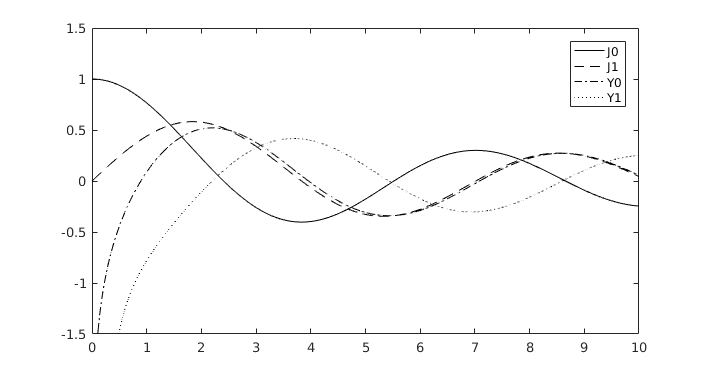
\includegraphics[width=\textwidth]{bessel.png}
						\caption{les deux premières fonctions de bessel de première et seconde espèces}
						\label{bessel}
					\end{figure}
				\end{center}
				
			
			Nous avons donc B = 0 puisque notre solution doit rester finie en r = 0.
			
			\begin{myrem}
				Dans le cas où l'origine ne ferait pas partie du domaine on ne peut négliger les fonctions Y
			\end{myrem}
			
			La condition $u(a,\theta,0) = 0$ se traduit par 
			
			$$J_{m}(ka) = 0$$
			$$k_{n}a = z_{mn}$$
			$$k_{mn} = \frac{z_{mn}}{a}$$
			
			Notre fonction $\phi$ devient alors
			
			$$\phi_{mn}(r,\theta) = J_{m} \left( \frac{z_{mn}}{a}r\right) (A \cos(m\theta) + B\sin(m\theta))$$
			
			\begin{myrem}
				$\phi_{mn}$ étant une fonction propre de Helmoltz, elle est orthogonale à $\phi_{ij}$
			\end{myrem}
			
			Pour calculer les coefficients nous devrons calculer des intégrales des fonctions de Bessel multiplier par une fonction. Lorsque cette fonction est un polynôme nous avons:
			
			$$\int x^{m} J_{0}(x) dx = x^{m} J_{1}(x) + (m-1)x^{m} J_{0}(x) - (m-1)^{2} \int x^{m-2} J_{0}(x)dx$$
			
	\subsection{L'équation de diffusion}
		L'équation de diffusion est de la forme
		
		$$\fpart{u}{t} = \alpha \ffpart{u}{x}$$
		
		Nous pouvons poser que
		
		$$u = R(x) + \Theta(x,t) $$
		
		Avec R(x) notre solution de régime et $\Theta(x,t)$ notre solution transitoire. Nous allons d'abords nous intéresser a notre solution de régime qui correspond à $\lambda =0$.
		
		$$ R_{0}''(x) = 0 \text{ et } T_{0}'(t) = 0$$
		
		Notre temps ne variant pas, nous sommes bien dans notre solution en régime.
		
		$$R_{0}(x) = A_{0} x + B$$
		
		En utilisant nos conditions limites, nous pouvons déterminer $A_{0}$ et $B_{0}$
		
		Nous nous intéressons maintenant à $\lambda = -K^{2}$ mais d'abord posons
		
		$$\Theta(x,\theta) = X(x) T(t)$$
		
		$$\frac{1}{\alpha} \frac{T'}{T} = \frac{X''}{X} = -K^{2}$$
		
		Nous obtenons pour T
		
		$$T(t) = C \exp(-\alpha K^{2}t)$$
		
		Et pour X
		
		$$X(x) = A \cos(Kx) + B \sin(Kx)$$
		
		En utilisant les conditions limites X(0) = X(L) = 0 étant donnée que nous avons aussi notre solution de régime
		
		$$ u(x,t) = R(x) + T(t) X(x)$$
		$$ T(t) X(x) = u(x,t) - R(x) $$
		$$ X(0) = u(0,t) - R(0) = 0 \text{ et }X(L) = u(L,t) - R(L) = 0$$
		
		Nous arrivons alors à
		
		$$X(x) = B sin(\frac{n\pi }{L}x)$$
		
		Et donc notre solution transitoire
		
		$$\Theta(x,t) = C sin(\frac{n \pi }{L}x) \exp(-\alpha K^{2})$$
		
		En utilisant notre condition initial pour trouver notre B nous avons
		
		$$R(x) + \sum_{n = 1}^{\infty} B_{n} sin(\frac{n \pi }{L}x)) = f(x)$$
		$$\sum_{n = 1}^{\infty} B_{n} sin(\frac{n \pi }{L}x)) = f(x) - R(x)$$
		$$ B_{n} \int_{0}^{L} \sin(\frac{n \pi}{L}x)^{2} dx = \int_{0}^{L} (f(x)-g(x)) \sin(\frac{n \pi}{L}x) dx$$
		$$ B_{n} =\frac{2}{L} \int_{0}^{L} (f(x)-g(x)) \sin(\frac{n \pi}{L}x) dx$$
		
		Il faut faire attention de ne pas oublier la solution de régime qui fais partie intégrante de la solution.
		
		
			


% TODO : équation de diffusion par séparation de variable.

\part{Analyse complexe}
\section{Rappels}
\begin{mydef}[Nombre complexe]
	Un nombre complexe $z$ est un couple de réels $(x,y) \in \mathbb{R}^2$ qui s'écrit
	sous la forme $z=x+iy$ où $x$ est la partie réelle de $z$ et $y$
	sa partie imaginaire. Un nombre complexe $z$ peut se représenter
	dans le plan complexe $\mathbb{R}^2$ (aussi appelé plan de Gauss).
	Dans cette représentation, $z$ est assimilé à un vecteur qui va de
	l'origine au point $(x,y)$. On peut écrire $z$ en notation polaire
	dans ce plan :
	\[z = x+iy = (x,y) = (r\cos\theta, r\sin\theta) = r\cos\theta + i r\sin\theta\]
	On définit alors
	\begin{itemize}
	    \item le module : la norme du vecteur $(x,y)$
	    \[|z| \triangleq r = \sqrt{x^2+y^2}\]
	    \item la phase (ou argument) : l'angle (orienté) entre le vecteur
	    et l'axe $\mathbb{R}_+$
	    \[arg(z) \triangleq \theta = \Atan(y, x)\footnotemark.\]
	        \footnotetext{\url{http://fr.wikipedia.org/wiki/Atan2}}
	\end{itemize}

\end{mydef}

\begin{mydef}[Argument principal $\Arg(z)$]
	L'argument d'un nombre complexe $z$ est défini à $2k\pi$ près, où
	$k$ est entier. On a en effet $\arg(z) = \theta_0 + 2k\pi$. On définit aussi
	$\Arg(z)$ qui retourne l'argument \textit{principal} de $z$,
	c'est à dire tel que $\theta_0 \in [-\pi;\pi[$.
\end{mydef}

\begin{mydef}[Nombre complexe conjugué]
	Le complexe conjugué d'un nombre $z = x+iy$ est noté:
	$$\bar{z} = x - iy$$
\end{mydef}

\begin{mydef}[Exponentielle complexe]\label{def:expComp}
	\[z = re^{i\theta} \triangleq r(\cos\theta+i\sin\theta)\]
	Ce qui est une autre écriture courante pour un complexe $z$.
\end{mydef}

\begin{mydef}[Fonctions trigonométriques]
	A partir de la définition \ref{def:expComp}, nous pouvons réécrire les fonctions trigonométriques comme:
	\begin{align*}
		&\cos(z) = \frac{e^{iz} + e^{-iz}}{2}
		&\sin(z) = \frac{e^{iz} - e^{-iz}}{2i}
	\end{align*}
\end{mydef}

\begin{mydef}[Fonctions Hyperboliques]
	\begin{align*}
		&\cosh(z) = \frac{e^{z} + e^{iz}}{2}
		&\sinh(z) = \frac{e^{z} - e^{-z}}{2}
	\end{align*}
\end{mydef}

\section{Fonctions d'une variable complexe}
\begin{mydef}[Fonction d'une variable complexe]
	Une fonction $f$ d'une variable complexe $z=x+iy$ incluse dans
	le domaine $D$ de $f$ est une application qui associe à tout
	élément $z$ de $D$ une image $f(z) = P(x,y) + iQ(x,y)$ où
	$P$ et $Q$ sont deux fonctions à deux variables réelles.
	Pour représenter une telle fonction, on utilise un
	graphe représentant la partie réelle et un graphe
	représentant la partie imaginaire.
\end{mydef}

\begin{mydef}
	Une fonction complexe $f(z)$ qui associe à un élément de son
	domaine $D$ plusieurs images est dite multiforme\footnote{Il
	ne s'agit donc plus à proprement parler d'une fonction.}. Dans
	le cas contraire, $f$ est dite uniforme.
\end{mydef}

\begin{mydef}\label{def:log}
	La fonction logarithme complexe se définit comme\footnote{Dans cette
	définition, il est important de distinguer le logarithme complexe
	du logarithme réel.}
	$$\log(z) \eqdef \log|z| + i\arg(z) = \log r + i(\theta_0 + 2k\pi)$$
	où $k$ est un entier. On remarque facilement que pour un même $z$,
	cette fonction a plusieurs images (l'argument étant défini à $2k\pi$
	près), $\log(z)$ est donc multiforme.
\end{mydef}

Sur base de cette définition, on peut généraliser l'exponentielle
complexe (qui est donc également une fonction multiforme).
\[z^a \eqdef e^{a\log z}\]


\begin{mydef}[Point de branchement]
	Soit une fonction complexe $f(z)$,
	le point $a$ est un point de branchement de $f$ lorsque
	l'image par $f$ d'au moins un lacet\footnote{C'est à dire un chemin
	continu fermé.} entourant $a$ est une courbe non fermée.
\end{mydef}

\begin{myprop}
    Si $f$ est une fonction complexe qui possède un
    point de branchement en $a$, alors
    \begin{itemize}
        \item $f$ est une fonction multiforme;
        \item $a$ est un point singulier.
    \end{itemize}
\end{myprop}

Intuitivement, on voit qu'en \og faisant un tour \fg autour d'un point
de branchement, on ne \og retrouve \fg pas la même image.

Par exemple, la fonction $\log$ possède un point de branchement
en $0$ (voir définition \ref{def:log}).
Cela découle directement du fait que la fonction $\arg$ est elle-même
multiforme et possède un point de branchement en $0$.

Les fonctions multiformes sont courantes
(toutes les fonctions qui sont définies par rapport au logarithme)
et ne sont pas faciles à traiter avec les outils usuels.
On cherche donc à les simplifier pour les rendre uniformes, tout en
gardant un maximum de leurs propriétés. Pour cela, une des techniques
est la définition de branches.

\begin{mydef}[Branche]
    Une branche (ou \emph{détermination}) d'une fonction
    multiforme $f$ définie sur un domaine $D$
    est une fonction uniforme $f^*$ définie sur $D$, qui prend une des valeurs
    de $f$ et qui est continue sur $D$, sauf sur une ou plusieurs courbes
    appelées \emph{coupures}.
\end{mydef}

Les différentes branches sont \og collées \fg entre elles par la coupure :
on \og passe \fg de l'une à l'autre par \og continuité \fg au niveau de la
coupure.

Par exemple, dans le cas du logarithme complexe,
une branche est un ensemble d'images correspondant à un même $k$.
La branche détermine dans ce cas une valeur unique pour la fonction argument
(d'où la valeur unique pour le logarithme), et la coupure est l'endroit ou
l'argument \og passe\fg d'une valeur à une autre (par exemple de $\pi$ à $-\pi$).

La \emph{surface de Riemann} du logarithme (fig. \ref{fig:riemann-log})
montre bien cela : le point de branchement est \og l'origine \fg des différentes
branches (\og feuilles \fg ou \og niveaux \fg dans la surface de Riemann).
Pour déterminer les branches, il faut choisir une coupure, ce qui découpe la surface
de Riemann en branches. Ainsi, sur chaque branche (que l'on peut définir par un
un intervalle de taille $2\pi$ pour $k$), la fonction est continue, sauf sur la coupure.

\begin{figure}
	\centering
		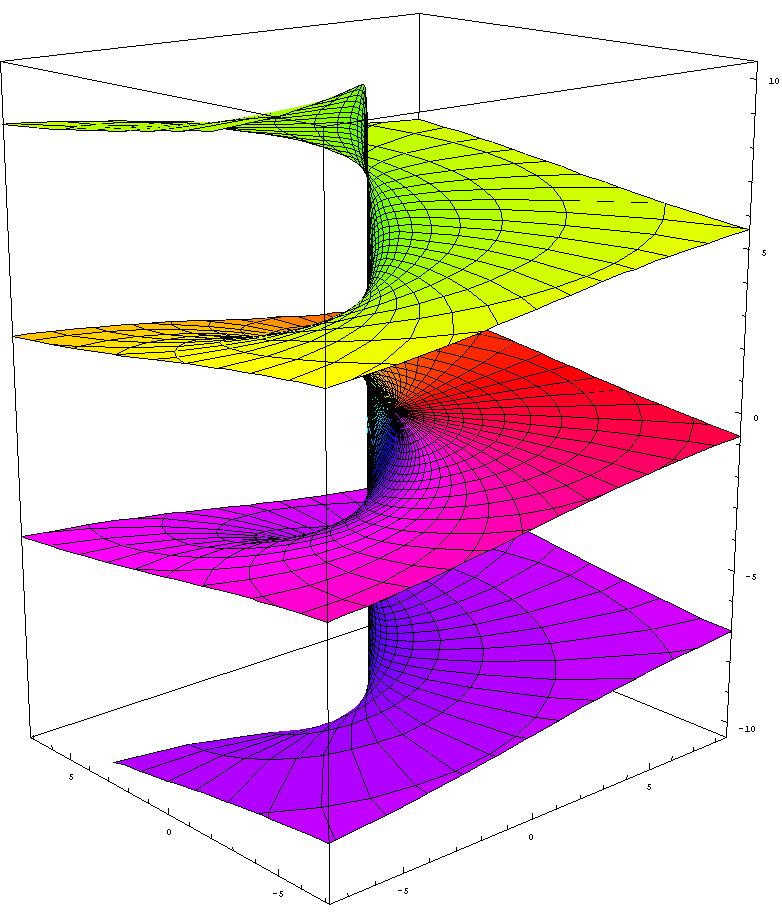
\includegraphics[width=0.3\textwidth]{riemann_surface_log.jpg}
		\caption{Illustration des concepts de point de branchement et
		de branche avec la surface de Riemann pour le logarithme complexe.
		L'origine (l'axe de l'escalier en colimaçon) est un point de branchement
		tandis que les différents étages de l'escalier correspondent à des branches.
		L'effet d'une coupure sur ce graphe serait de ne garder qu'un seul étage
		(une seule branche). On remarque que la fonction deviendrait alors discontinue.}
		\label{fig:riemann-log}
\end{figure}

\begin{myrem}
	Pour trouver les points de branchements d'une fonction complexe
	$f(z)$, on procède comme suit :
	\begin{enumerate}
		\item On fait apparaître le(s) logarithme(s) caché(s) dans
		l'expression de $f$ ;
		\item	Les points qui annulent l'argument du ou des logarithmes
		sont des candidats point de branchement ;
		\item On vérifie que ces candidats sont bien des points
		de branchement en ``tournant'' autour des ces points
		et en observant si $f$ prend plusieurs valeurs différentes
		pour des points de départs identiques (mais dont l'argument
		diffère de $k2\pi$).
	\end{enumerate}
	En effet, toutes les fonctions courantes qui ont des points
	de branchement peuvent être définies sur base du logarithme complexe.
	Il suffit donc de développer l'expression pour trouver les points
	de branchement.
\end{myrem}

\begin{mydef}[Coupure canonique et branche principale]
    Pour les fonctions usuelles, on a un choix par défaut
    de coupure : la coupure canonique.

    Pour cette coupure, on choisit une branche par défaut,
    la branche principale. La branche principale est souvent choisie
    pour que la fonction puisse se restreindre de façon classique à la
    fonction réelle correspondante.
\end{mydef}

\begin{myrem}
    La branche principale de $\log(z)$ correspond à un argument
    $\theta\in [-\pi, \pi[$. On remarque que pour $z = r \in \mathbb{R}$,
    $\log(z) = \ln(r)$.

    Le fonction logarithme restreinte à sa branche principale est
    appelée \emph{logarithme principal} et notée $\Log$.

    La même idée est appliquée à la fonction argument,
    avec l'\emph{argument principal} $\Arg(z) \in [-\pi, \pi[$.

    On a alors
    \[\Log(z) \eqdef \log|z| + i\Arg(z) = \log r + i\theta_0\]
    avec $\theta_0 \in [-\pi,\pi[$.
\end{myrem}

Le nombre de branches issues d'un point de branchement est égal au
nombre de tours qu'il faut faire autour du point de branchement pour
retrouver une même valeur. Pour la racine $n$-ième, ce nombre vaut $n$,
pour le logarithme, il n'existe pas.

\begin{myexem}\label{ex:branches1}
    Soit $f(z) = \sqrt{z(z-1)}$, recherchons
    les points de branchement, coupures et branches.
    On exprime la fonction comme
    \[f(z) = e^{\frac{1}{2}\log(z(z-1))}\]
    Les candidats points de branchement sont $0$ et $1$.
    Pour simplifier, notons $z = r_1 e^{i\theta_1}$ et
    $z-1 = r_2 e^{i\theta_2}$.
    On a \[f(z) = \sqrt{r_1 r_2} e^{i\frac{\theta_1+\theta_2}{2}}\]
    Dès lors, on peut voir que $0$ et $1$ sont bien des points
    de branchement : si on remplace $\theta_1$ (argument associé
    au point $0$) par $\theta_1 + 2\pi$, on obtient une valeur
    différente, et c'est pareil pour $\theta_2$.
    On peut définir des coupures. Ce choix est arbitraire, trois
    exemples sont représentés sur la figure \ref{fig:branches1}.
    Dans le cas général ($\mathcal{A}$ et $\mathcal{B}$),
    il faut une coupure qui part de chaque point
    de branchement et les coupures continuent à l'infini.
    Dans le cas $\mathcal{C}$, la coupure relie les deux points de
    branchement et ne va pas à l'infini.\footnote{
        Cela est possible car la fonction n'a pas de point de
        branchement à l'infini. On peut également le voir en constatant
        qu'il n'y a pas \og globalement \fg de point de branchement
        si on considère un lacet entourant $0$ et $1$ : son image est
        une courbe fermée.}

    \begin{figure}
    \centering
    \begin{tikzpicture}[scale=0.2]
    \coordinate (point) at (20, 10);
    \draw[<->] (0, 12) -- (0, 0) -- (22, 0);
    \draw[->] (0, 0) -- (point) node[midway, above] {$r_1$};
    \draw[->] (10, 0) -- (point) node[midway, right] {$r_2$};
    \draw (4, 0) arc (0:26.5:4) node[midway, right] {$\theta_1$};
    \draw (14, 0) arc (0:45:4) node[midway, right] {$\theta_2$};
    \draw[red,ultra thick, dashed] (0, 0) -- (-5, 0) node[midway, below] {$\mathcal{A}_1$};
    \draw[red,ultra thick, dashed] (10, 0) -- (22, 0) node[midway, below] {$\mathcal{A}_2$};
    \draw[blue,ultra thick, dashed] (0, 0) -- (-5, 10) node[midway, left] {$\mathcal{B}_1$};
    \draw[blue,ultra thick, dashed] (10, 0) -- (8, -5) node[midway, right] {$\mathcal{B}_2$};
    \draw[green,ultra thick, dashed] (0, 0) -- (10, 0) node[midway, below] {$\mathcal{C}$};
    \end{tikzpicture}
    \caption{Différents choix de coupures pour la fonction $f(z) = \sqrt{z(z-1)}$
        (voir exemple \ref{ex:branches1}).}
    \label{fig:branches1}
    \end{figure}
\end{myexem}

\subsection{Limites et dérivées}
On a une définition semblable pour la limite et la continuité
pour $f(z)$ que pour les fonctions à plusieurs variables
\begin{mydef}[Limite]
  $\lim_{z\to z_0} f(x) = L$ si et seulement si
  \[ \forall \epsilon>0, \exists\delta>0:
  |z-z_0|<\delta \Rightarrow |f(z)-L|<\epsilon. \]
\end{mydef}
\begin{mydef}[Continuité]
  $f$ est continue en $z_0$ si et seulement si $f$ est définie en $z_0$ et
  \[ \lim_{z \to z_0} f(z) = z_0. \]
\end{mydef}

La définition de la dérivée par contre, est fort différente
et c'est là que réside tout l'intérêt de l'analyse complexe.
En effet, pour les fonctions à plusieurs variables, le dénominateur est
équivalent à $|z - z_0|$ alors qu'ici, c'est $z - z_0$.
\begin{mydef}
  \[ f'(z_0) = \lim_{z \to z_0} \frac{f(z) - f(z_0)}{z - z_0}. \]
\end{mydef}

En pratique, les fonctions usuelles sont continues et dérivables si
on défini les coupures correctement et les règles de dérivations
habituelles sont aussi vérifiées.
Par exemple, $f(z) = z^2$ est continue et dérivable pour tout $z$ et
$f'(z) = 2z$.
Par contre la fonction conjugué $f(z) = \bar{z}$ n'est pas dérivable.

On définit d'ailleurs deux nouveaux termes
\begin{mydef}
  Une fonction $f(z)$ holomorphe est une fonction définie et dérivable
  en tout point d'un sous-ensemble ouvert du plan complexe.
\end{mydef}
\begin{mydef}
  Une fonction $f(z)$ entière est une fonction holomorphe sur tout
  le plan complexe.
\end{mydef}

Comme $f(z)$ a une image complexe,
on peut définir $P$ et $Q$ comme suit $f(z) = P(z) + iQ(z)$.
Définissons aussi $x$ et $y$ comme suit $z = x + iy$.
On a alors le théorème suivant.
\begin{mytheo}[Condition de Cauchy-Riemann]
  $f$ est différentiable si et seulement si
  \[ \left\{\begin{aligned}
      \fpart{P}{x} & = \fpart{Q}{y}\\
      \fpart{Q}{x} & = -\fpart{P}{y}.
  \end{aligned}\right. \]
\end{mytheo}

Un corolaire direct de ce théorème, c'est que $f$ respecte l'équation
de Laplace $\lap f = 0$.
En effet, on obtient sans mal $\lap P = 0$ et $\lap Q = 0$ d'où
$\lap f = \lap P + i\lap Q = 0$.

\begin{mytheo}
	Soit $f(z)$ holomorphe dans un domaine $D$
    et $C \subseteq D$ un contour fermé entourant $z$.
    À partir de la formule intégrale
	de Cauchy (théorème \ref{thm:int}),
	on peut démontrer la formule suivante
	\[ f^{(n)}(z) = \frac{n!}{2\pi i}\oint_C
	\frac{f(\xi)}{(\xi-z)^{n+1}}\dif \xi.\]
\end{mytheo}

\subsection{Intégrales}
L'intégrale complexe a une définition essentiellement identique à
l'intégrale réelle :

\begin{mydef}[Intégrale complexe sur un chemin]
    Soit un chemin $C$ allant de $a$ à $b$ ($a, b \in \mathbb{C}$)
    \[\int_a^b f(z) \dif z =
    \lim_{S \to 0} \sum_{k=1}^{n} f(\xi_k)(z_k - z_{k-1})\]
    Avec
    \begin{itemize}
        \item $(z_k)_{k = 0, 1, ..., n}$ une suite ordonnée d'éléments
            de $C$ telle que $z_0 = a$ et $z_n = b$
        \item $\xi_k$ un élément de $C$ situé entre $z_{k-1}$ et $z_k$
        \item $S = \max_{k = 1, ..., n}(|z_k - z_{k-1}|)$
    \end{itemize}
\end{mydef}


Cauchy-Riemann nous permet de montrer
une théorème fort intéressant concernant les intégrales baptisé le
théorème de Cauchy.
\begin{mytheo}[Théorème de Cauchy]
  Soit $f(z)$ holomorphe dans un domaine $D$ ``simplement connexe''
  avec $C \subseteq D$.
  On a
  \[ \oint_C f(z) \dif z = 0. \]
\end{mytheo}
De ce dernier, on peut montrer la formule intégrale de Cauchy.
\begin{mytheo}[Formule intégrale de Cauchy]
  \label{thm:int}
  Soit $f(z)$ holomorphe dans un domaine $D$
  avec $C \subseteq D$. % fermé simple
  On a
  \[ f(z) = \frac{1}{2\pi i}\oint_C
  \frac{f(\zeta)}{\zeta-z} \dif \zeta \]
  où on parcourt $C$ \strong{dans le sens trigonométrique}
  \footnote{i.e. le sens anti-horlogique.}.
  En effet, si cette formule était indépendante du sens,
  ça n'aurait pas de sens,
  en changeant le sens de l'intégrale,
  on doit avoir $-f(z)$.
  C'est le sens trigonométrique ici car c'est dans ce sens
  là qu'on mesure les angles orientés et que les angles en trigonométrie
  sont orientés.
  En effet, $\dif \theta$ est positif si on tourne dans le sens
  trigonométrique et négatif sinon.
\end{mytheo}

Cette formule permet déjà de calculer certaines intégrales mais
en fait, ce n'est qu'un \emph{cas particulier} du théorème des Résidus.
En effet, on verra que $z$ est ici un pôle d'ordre 1 de
$g(\zeta)=\frac{f(\zeta)}{\zeta-z}$
et $f(z)$ est alors son résidu en $z$ noté
$\res(g,z)$.
Toutes les intégrales qui peuvent se calculer avec la formule
intégrale de Cauchy peuvent donc être calculée avec le théorème
des Résidus.

\begin{mytheo}[Théorème des Résidus]
  Soit $D$ un domaine simplement connexe avec
  $C \subseteq D$ et $f$ analytique
  sauf en certains pôles $z_1, z_2, \ldots, z_n$.
  On a
  \[ \oint_C f(z) \dif z = 2i\pi\sum_{k=1}^n \res(f, z_k). \]
  À nouveau,
  comme pour le théorème~\ref{thm:int},
  $\oint_C$ doit être dans le sens trigonométrique sinon,
  il y a un signe $-$ dans le membre de droite de l'équation.
\end{mytheo}

Il y a deux nouveaux points à aborder pour comprendre ce théorème
``magique''.
Qu'est-ce qu'un pôle et comment calculer un résidu.

Supposons qu'on ait une singularité $z_0$.
Elle peut être
\begin{itemize}
  \item soit ``effaçable'', ça veut dire que $f$ reste borné en $z_0$
	(exemple\footnote{On peut facilement vérifier que le pôle
	de cet exemple est effaçable en calculant le développement
	en série de Taylor de $f(z)$.} : $f(z) = \frac{\sin(z-z_0)}{z-z_0}$) ;
  \item soit un pôle, ça veut dire que $f$ tend vers l'infini en $z_0$;
  \item soit essentielle, ça veut dire que la limite n'existe pas en $z_0$
	(exemple : $f(z) = \sin(\frac{1}{z})$).
\end{itemize}

L'idée du théorème des Résidus, c'est que $\oint_C f(z) \dif z$ ne vaut
pas 0 mais $2i\pi$ fois la somme des
$\frac{1}{2i\pi} \oint_{C_k} f(z) \dif z$ qu'on
nomme $\res(f, z_k)$.
Il suffit donc de calculer ces intégrales.

Pour cela, introduisons un développement en série plus générale qui
part de $-\infty$.
\begin{mydef}[Développement en série de Laurent]
  Soit $f$ analytique sur $D \subseteq \mathbb{C}$,
  le développement en série de Laurent de $f$ autour de $a$ est
  \[ f(z) = \sum_{-\infty}^{\infty}b_n(z-z_0)^n. \]
\end{mydef}
L'avantage de ce développement en série, c'est que
$\oint_C (z-z_0)^j$ est nul pour tout $j \neq -1$ et vaut $2\pi i$ si
$j = -1$.

Le développement de Taylor est le cas particulier de ce développement
pour $f$ analytique.
Ici, $f$ n'est pas analytique car il a un pôle.
L'astuce c'est que pour tout pôle, il existe un plus petit entier
$m$ tel que $H = (z-z_k)^mf$ est analytique sur $C_k$.
On dit alors que $z_k$ est un pôle à l'ordre $m$.

On peut alors calculer Taylor pour $H$ en $z_k$,
le diviser par $(z-z_k)^m$ et ça donne le développement en série de Laurent
de $f$.
En intégrant ce développement en série, on a vu plus haut,
qu'il n'y avait que $b_{-1}$ qui restait,
c'est à dire $c_{m-1}$ dans le développement en série de Taylor de
$H$.
On a donc
\begin{align*}
  b_{-1} & = c_{m-1}\\
  & = \frac{1}{(m-1)!}\lim_{z\to z_k} H^{(m-1)}(z)\\
  & = \frac{1}{(m-1)!}\lim_{z\to z_k} \fdif{^{m-1}}{z^{m-1}}
  \left((z-z_k)^m f(z)\right).
\end{align*}

\begin{mydef}[Résidu d'une fonction]
  Le résidu d'une fonction $f$ avec un pôle de degré $n$ en $a$ est
  $\res_a f = b_{-1}$.
  Il peut également être obtenu par la formule suivante
  \[ \res_a f = \frac{1}{(n-1)!} \lim_{z \to a}
  \fdif{^{n-1}}{z^{n-1}}((z-a)^nf(z)) \]
\end{mydef}

On peut maintenant calculer des intégrales très compliquées à l'aide de
deux lemmes.
\begin{mylem}[Lemme de Jordan I]
  Soit $f$ analytique sur $D \subseteq \mathbb{C}$.
  Si $\lim_{|z|\to\infty} |zf(z)| = 0$, alors
  \[ \lim_{R\to\infty} \oint_{C(0,R,\alpha)}f(z)\dif z = 0. \]
\end{mylem}
\begin{mylem}[Lemme de Jordan III]
  Soit $f$ analytique sur $D \subseteq \mathbb{C}$.
  Si $\lim_{|z|\to 0} |zf(z)| = 0$, alors
  \[ \lim_{R\to 0} \oint_{C(0,R,\alpha)}f(z)\dif z = 0. \]
\end{mylem}

\begin{mydef}[transformation complexe]
	Une fonction complexe $Z = X + IY = P(x,y) + iQ(x,y) $ peut être regardée comme une transformation du plan complexe z en le plan complexe Z.
\end{mydef}

\begin{myprop}
	La transformation est bijective dans les domaines où son jacobien est nul.
\end{myprop}

\begin{myprop}
	Si la transformation $f(z)$ est holomorphe dans un domaine D et telle que $f'(z) \neq 0$, alors la transformation inverse $f^{-1}$ est définie et holomorphe en tout point du transfom de D par f.
\end{myprop}

\begin{mydef}[Transofmation conforme]
	On appelle transformation conforme une transformation qui conserve les angles en grandeur et en sens.
\end{mydef}

\begin{mydef}[Transformation de Scharwz-Christoffel]
	Soit un polygone dans le plan Z ayant pour sommets les points $Z_{1},Z_{2}, \ldots,Z_{n}$ et pour angles intérieurs $\alpha_{1},\alpha_{2}, \ldots,\alpha_{n}$. Soient les points $x_{1},x_{2}, \ldots,x_{n}$ de l'axe réel du plan z. Une transformation qui fait correspondre au plan $y\geq 0$ du plan z, l'intérieur du polygone du plan Z, les points $x_{i}$ correspondant aux $Z_{i}$, est donné par l'équation:
	
	$$\frac{dZ}{dz} = A (z-x_{1})^{\cfrac{\alpha_{1}}{\pi}-1} (z-x_{2})^{\cfrac{\alpha_{2}}{\pi}-1} \ldots (z-x_{n})^{\cfrac{\alpha_{n}}{\pi}-1}$$
\end{mydef}

\begin{myrem}
	La transformation de Scharwz-Christoffel n'est pas conforme aux points anguleux du polygone
	\end{myrem}

\annexe
\section{Dirac}
\label{app:dirac}
Un Dirac est une fonction avec singularité en 0.
Elle se note $\delta(x)$ et est définie par
\begin{equation}
  \label{eq:dirac1}
  \delta(x) =
  \begin{cases}
    \infty, & x = 0\\
    0, & x \neq 0
  \end{cases}
\end{equation}
et
\begin{equation}
  \label{eq:dirac2}
  \int_{-\infty}^{\infty} \delta(x) \dif x = 1.
\end{equation}

Ça peut paraitre bizarre que l'intégrale soit finie alors que
$\delta(0) = \infty$.
Seulement, rappelez vous qu'une intégrale c'est une aire et que
l'aire d'un Dirac n'est pas entièrement définie par \eqref{eq:dirac1}
car celle ci impose que l'aire vaut $0 \cdot \infty$ qui est un cas
d'indétermination.
\eqref{eq:dirac2} permet de lever cette indétermination.

\end{document}
